% Just The Docs Front Matter
% title: Mesh Generation
% parent: Capabilities
% has_children: false
% has_toc: false

\subsection{Mesh Generation} \label{sec:using-issm-capabilities-mesh-generation}
\subsubsection{ARGUS file format}%{{{
To mesh the domain, one needs a file containing all the coordinates of the domain outline in an \href{http://www.argusint.com/}{ARGUS} format. These files have a \lstinlinebg|*.exp| extension. Here is an example of such a file for a square glacier:
\begin{lstlisting}
## Name:DomainOutline
## Icon:0
# Points Count  Value
5 1.000000
# X pos Y pos
0 0
1000000 0
1000000 1000000
0 1000000
0 0
\end{lstlisting}
The ARGUS format is used extensively by ISSM. One can use \lstinlinebg|exptool| to generate and manage \href{http://www.argusint.com/}{ARGUS} files.
%}}}
\subsubsection{triangle}%{{{
\lstinlinebg|triangle| is a wrapper of \href{http://www.cs.cmu.edu/~quake/triangle.html}{triangle} developed by \href{http://www.cs.berkeley.edu/~jrs/}{Jonathan Shewchuk} \citep{Shewchuk1996}. It generates unstructured isotropic meshes:
\begin{lstlisting}
>> md = triangle(md, 'DomainOutline.exp', 5000);
\end{lstlisting}
The first argument is the model you are working on, the second argument is the file from ARGUS containing the domain outline, and the last argument is the density of the mesh (the mean distance between two nodes). To see what the mesh looks like, one can run:
\begin{lstlisting}
>> plotmodel(md, 'data', 'mesh');
\end{lstlisting}
\begin{figure}[H]
	\begin{center}
		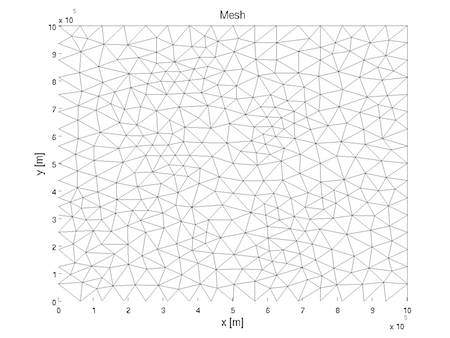
\includegraphics[width=\textwidth]{\assetsParentPath/assets/img/using-issm/capabilities/mesh/mesh.png}
		\caption{Mesh}
	\end{center}
\end{figure}

ISSM includes a mesh adaptation capability embedded in the code, inspired by \href{https://people.math.sc.edu/Burkardt/data/bamg/bamg.html}{BAMG} developed by Frederic Hecht \citep{Hecht2006}, and YAMS developed by Pascal Frey \citep{Frey2001}.
%}}}
\subsubsection{Bamg}%{{{
\paragraph{Domain}
To mesh the domain, you need a file containing all the coordinates of the domain outline in an ARGUS format. Assuming that this file is \lstinlinebg|DomainOutline.exp|, run:
\begin{lstlisting}
>> md = bamg(md, 'DomainOutline.exp');
\end{lstlisting}

\paragraph{hmin/hmax}
The minimum and maximum edge lengths can be specified by \lstinlinebg|'hmin'| and \lstinlinebg|'hmax'| options:
\begin{lstlisting}
>> md = bamg(md, 'DomainOutline.exp', 'hmax', 1000);
\end{lstlisting}

\paragraph{hVertices}
One can specify the edge length of domain outline vertices. Use \lstinlinebg|NaN| if an edge length value is not required/available:
\begin{lstlisting}
>> h = [1000 100 100 100];
>> md = bamg(md, 'DomainOutline.exp', 'hmax', 1000, 'hVertices', h);
\end{lstlisting}

\paragraph{field/err}
The option \lstinlinebg|'field'| can be used with the option \lstinlinebg|'err'| to generate a mesh adapted to the field given as input for the error given as input:
\begin{lstlisting}
>> md = bamg(md, 'field', md.inversion.vel_obs, 'err', 1.5);
\end{lstlisting}
Multiple fields can also be used:
\begin{lstlisting}
>> md = bamg(md, 'field', [md.inversion.vel_obs md.geometry.thickness], 'err', [1.5 20]);
\end{lstlisting}

\paragraph{gradation}
The ratio of the lengths of two adjacent edges is controlled by the option \lstinlinebg|'gradation'|:
\begin{lstlisting}
>> md = bamg(md, 'field', md.inversion.vel_obs, 'err', 1.5, 'gradation', 3);
\end{lstlisting}

\paragraph{anisomax}
The factor of anisotropy (ratio between the lengths of two edges belonging to the same triangle) can be changed by the option \lstinlinebg|'aniso'|. A factor of anisotropy equal to 1 will result in an isotropic mesh generation:
\begin{lstlisting}
>> md = bamg(md, 'field', md.vel_obs, 'err', 1.5, 'anisomax', 1);
\end{lstlisting}
NOTE: Users using Intel compilers (\lstinlinebg|icc|, \lstinlinebg|icpc|) shoud use the flag \lstinlinebg|-fp-model precise| to disable optimizations that are not value-safe on floating-point data. This will prevent bamg from being compiler dependent (see \href{https://software.intel.com/en-us/node/522979}{here}).

\subsubsection{Extrusion (3D)}
One can extrude the mesh, in order to use a three-dimensional model (Pattyn's higher order model and Full Stokes model). This step is not mandatory. If the user wants to keep a 2D model, skip this section.

To extrude the mesh, run the following command:
\begin{lstlisting}
>> md = extrude(md, 8, 3);
\end{lstlisting}
The first argument is the model, as usual. The second argument is the number of horizontal layers. A high number of layers gives a better precision for the simulations but creates more elements, which requires a longer computational time. Usually a number between 7 and 10 is a good balance. The third argument is called the extrusion exponent. Interesting things are usually happening near the bedrock and therefore users might want to refine the lower layers more than the upper ones. An extrusion exponent of 1 will create a mesh with layers equally distributed vertically. The higher the extrusion exponent, the more refined the base. An extrusion exponent of 3 or 4 is generally enough.
\begin{figure}[H]
	\begin{center}
		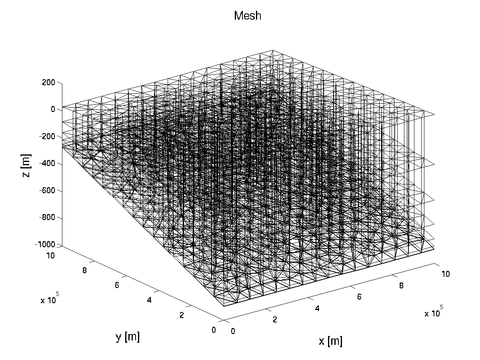
\includegraphics[width=\textwidth]{\assetsParentPath/assets/img/using-issm/capabilities/mesh/extrusion.png}
		\caption{Extruded mesh}
	\end{center}
\end{figure}
%}}}

\clearpage % Make sure all figures are placed before next section
